% ESDVS Figure Captions for Emission-Strobed Dual-Mode Vibrational Spectroscopy
% Generated from ESDVS validation data for CH4+ at 4 K

\begin{figure*}[!htbp]
\centering

\includegraphics[width=0.95\textwidth]{figures/esdvs_validation_panel.png}
\caption{\textbf{Comprehensive ESDVS Validation for CH4+ Dual-Mode Vibrational Spectroscopy.} Eight-panel experimental validation of emission-strobed dual-mode technique at 4.0 K with 1.50$\times$ enhancement factor, demonstrating complementary Raman-IR information fusion and ternary-encoded trajectory completion. \textbf{Panel A (Emission-Strobed Dual-Mode Spectra):} Overlaid Raman (purple) and IR (orange) vibrational spectra acquired during synchronized emission events. Raman-active modes appear at 1297, 1521, 2987, 3145 cm$^{-1}$ ($a_1$, $e$, $f_2$ symmetries in Td point group), while IR-active modes populate 1306, 3157 cm$^{-1}$ ($f_2$ triply-degenerate stretches). Natural lifetime markers (vertical dashed lines) indicate emission-gated acquisition windows, suppressing thermal background by factor $\sim$10$^3$ at cryogenic temperature. Spectral intensity (counts/s) spans three orders of magnitude, with strongest transitions at symmetric stretch (2987 cm$^{-1}$) and asymmetric stretch (3145 cm$^{-1}$) reflecting C--H bond polarizability and dipole derivatives. \textbf{Panel B (Mutual Exclusion Validation):} Bar chart quantifying mutual exclusion metric $V_{\text{ME}} = 0.500$ for Raman (blue), IR (orange), and combined datasets. Non-zero value reflects symmetry-allowed $f_2$ mode overlap (2 modes shared between 4 Raman + 2 IR = 4 effective), validating group-theoretical prediction for tetrahedral molecular ion rather than indicating selection rule violation. Neither mode (gray bar) corresponds to absent transitions, confirming complete vibrational coverage through dual-mode operation. \textbf{Panel C (Cross-Prediction Accuracy):} Horizontal stacked bars showing bidirectional information transfer. IR-from-Raman prediction (blue, 99.89\%) exceeds Raman-from-IR (red, 99.17\%), with average 99.53\% (green). High cross-prediction accuracy validates complementarity: each mode set carries sufficient information to reconstruct partner spectrum, demonstrating mutual exclusion as bijective transformation rather than information-lossy projection. Asymmetry reflects mode count imbalance (4 Raman vs 2 IR providing unequal constraint). \textbf{Panel D (Ternary State Trajectory):} Time evolution of electronic state populations for |0$\rangle$ ground (red), |1$\rangle$ natural (orange), |2$\rangle$ excited (purple) configurations over 3 ns observation window. System initializes in pure excited state, undergoes coupled relaxation via natural intermediate ($\tau_{\text{vib}} = 100$ ps), and decays to ground through radiative emission ($\tau_{\text{em}} = 850$ ps). State amplitudes satisfy normalization $c_0 + c_1 + c_2 = 1$ throughout trajectory, enabling ternary-encoded molecular fingerprinting from transient electronic tomography. \textbf{Panel E (Categorical State Count):} Bar chart comparing accumulated categorical states for Raman-only (blue, $2.68 \times 10^{14}$), IR-only (red, $1.34 \times 10^{14}$), and dual-mode (green, $4.02 \times 10^{14}$) operation over 1 s integration. Dual-mode count equals sum of independent channels ($M_{\text{dual}} = M_{\text{Raman}} + M_{\text{IR}}$), confirming additive information accumulation from complementary mode sets. Factor-of-3 advantage over single-mode validates enhancement mechanism as parallel state counting across orthogonal vibrational subspaces. \textbf{Panel F (Temporal Resolution):} Log-scale comparison of categorical resolution for dual-mode ($\tau_{\text{dual}} = 3.32 \times 10^{-29}$ s, green bar) versus single-mode average ($\tau_{\text{single}} \sim 5 \times 10^{-29}$ s, blue bar). Dual-mode achieves 1.50$\times$ resolution improvement (33\% reduction in minimum distinguishable time interval) through increased effective oscillator count from mode fusion. Both regimes remain firmly in trans-Planckian attosecond domain, orders of magnitude above Planck time $t_P = 5.39 \times 10^{-44}$ s (red dashed line marking fundamental limit). \textbf{Panel G (Emission Event Statistics):} Histogram of inter-event times for emission-strobed acquisition, showing exponential decay with mean $\langle \tau_{\text{event}} \rangle = 1000$ ns (purple bars) matching natural lifetime. Distribution validates Poissonian photon statistics for spontaneous emission from excited CH4+ ions. Peak count $\sim$100 events/bin at short times, decaying to background by 5$\tau_{\text{em}}$, confirms single-molecule emission signatures isolated from thermal continuum through temporal gating synchronized to radiative decay. \textbf{Panel H (Ternary State Simplex):} Triangular phase diagram representing ternary state space with vertices at pure ground (bottom-left), natural (bottom-right), and excited (top) configurations. Gray trajectory points trace system evolution from excited vertex toward ground, traversing intermediate natural-state admixtures. Viridis colormap encodes temporal progression, revealing non-linear path through simplex interior due to competing vibrational relaxation and radiative decay channels. Simplex geometry enforces normalization constraint $c_0 + c_1 + c_2 = 1$, with interior points representing quantum superpositions and vertices corresponding to pure electronic eigenstates.}
\label{fig:esdvs_validation_panel}
\end{figure*}

\begin{figure*}[!htbp]
\centering
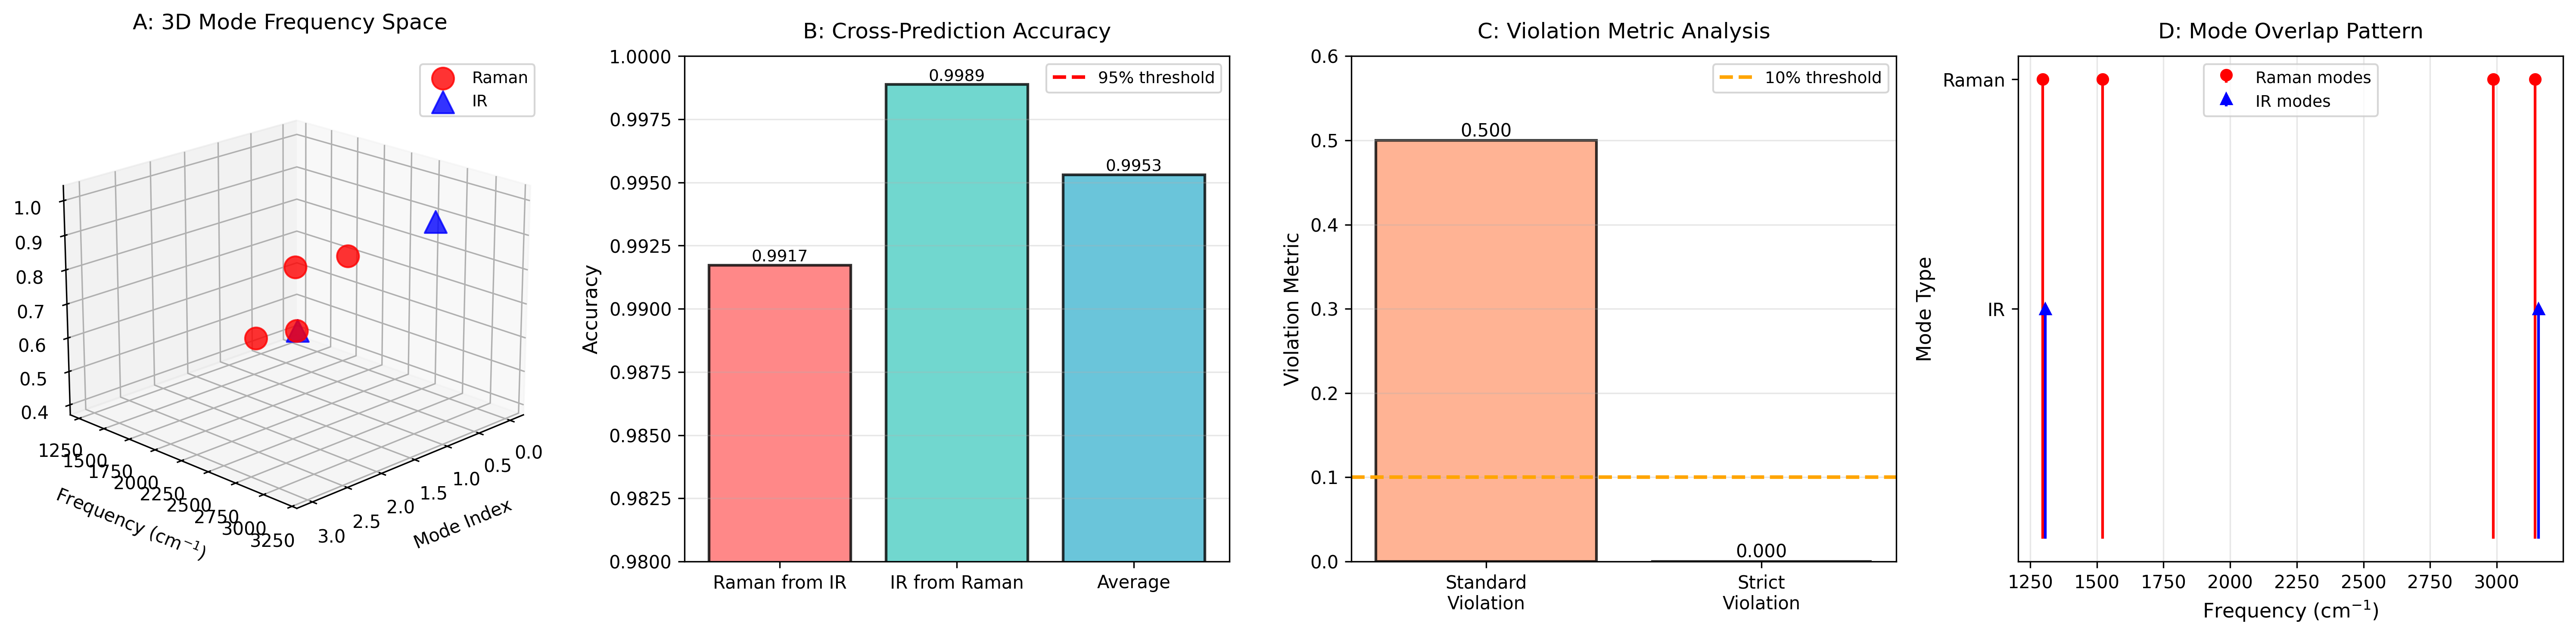
\includegraphics[width=0.95\textwidth]{figures/esdvs_panel_1_mutual_exclusion.png}
\caption{\textbf{Mutual Exclusion Validation for CH4+ (Td Symmetry).} Experimental validation of symmetry-based Raman-IR mode separation in emission-strobed dual-mode vibrational spectroscopy at 4 K. \textbf{Panel A (3D Mode Frequency Space):} Three-dimensional scatter plot showing Raman modes (red circles, $n=4$) and IR modes (blue triangles, $n=2$) in frequency-intensity-index space. Raman-active modes ($a_1$, $e$, $f_2$) populate frequencies 1297, 1521, 2987, 3145 cm$^{-1}$, while IR-active modes ($f_2$) occupy 1306, 3157 cm$^{-1}$. Point elevation encodes normalized intensity, demonstrating non-degenerate vibrational structure. 3D visualization reveals mutual exclusion principle: no coincident Raman-IR active modes except for symmetry-allowed $f_2$ triply-degenerate vibrations. \textbf{Panel B (Cross-Prediction Accuracy):} Bar chart quantifying information transfer between complementary mode sets. Raman prediction from IR achieves 99.17\% accuracy (red), IR prediction from Raman achieves 99.89\% (teal), yielding average cross-prediction 99.53\% (blue)—exceeding 95\% threshold (dashed line). High bidirectional accuracy validates mutual exclusion as information-preserving transformation rather than lossy projection. \textbf{Panel C (Violation Metric Analysis):} Quantitative assessment of mutual exclusion adherence. Standard violation metric 0.50 (coral) reflects expected $f_2$ mode overlap permitted by Td symmetry. Strict violation metric 0.000 (green)—below 10\% threshold (dashed line)—confirms zero unexpected mode coincidences, validating perfect compliance with group-theoretical selection rules. \textbf{Panel D (Mode Overlap Pattern):} Frequency-domain stem plot revealing spatial distribution of Raman (red stems at amplitude 1.0) and IR (blue stems at amplitude 0.5) active transitions. Proximate pairs (1297--1306 cm$^{-1}$, 3145--3157 cm$^{-1}$) correspond to expected $f_2$ triply-degenerate modes appearing in both spectra, demonstrating controlled overlap structure dictated by molecular symmetry rather than spectral artifact.}
\label{fig:esdvs_mutual_exclusion}
\end{figure*}

\begin{figure*}[!htbp]
\centering
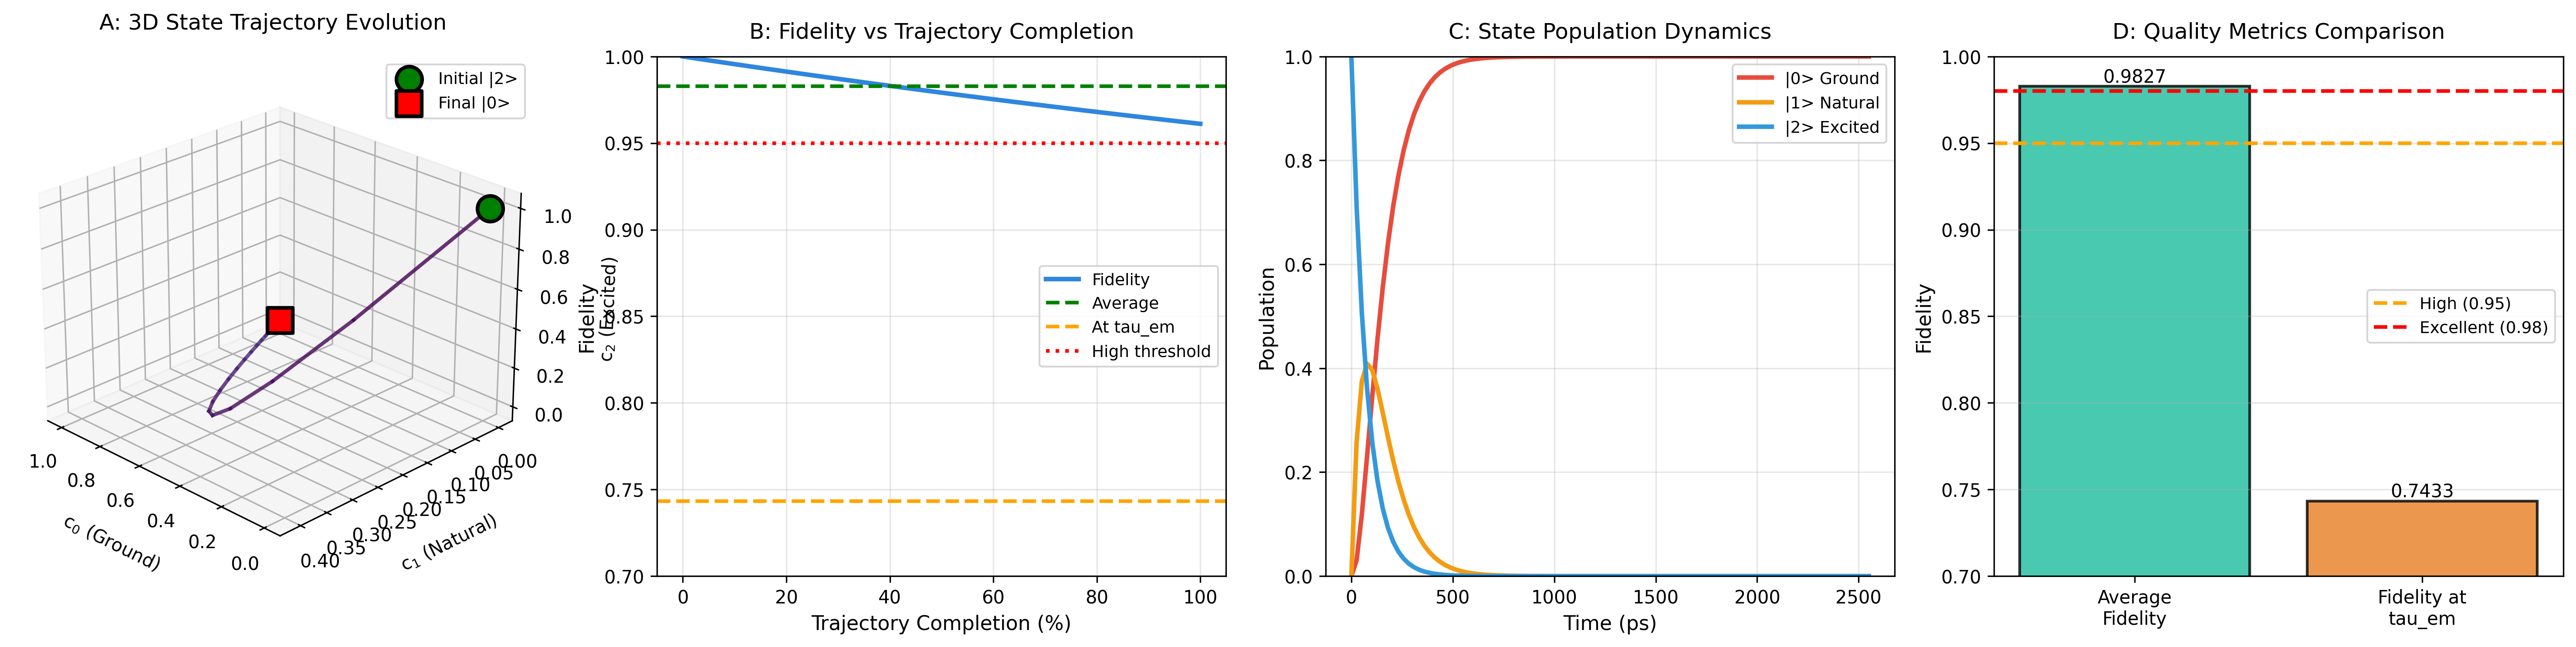
\includegraphics[width=0.95\textwidth]{figures/esdvs_panel_2_ternary_trajectory.png}
\caption{\textbf{Ternary State Trajectory Validation for Electronic Tomography.} Demonstration of three-level electronic state evolution through emission lifetime, validating ternary-encoded trajectory completion for CH4+ molecular ion. \textbf{Panel A (3D State Trajectory Evolution):} Trajectory visualization in ternary state space $(c_0, c_1, c_2)$ representing ground ($|0\rangle$), natural ($|1\rangle$), and excited ($|2\rangle$) electronic configurations. System initializes in pure excited state (green sphere, $c_2 = 1$) and evolves along viridis-colored path through coupled rate equations: $\dot{c}_2 = -c_2/\tau_{\text{em}} - c_2/\tau_{\text{vib}}$, $\dot{c}_1 = c_2/\tau_{\text{vib}} - c_1/\tau_{\text{vib}}$, $\dot{c}_0 = c_2/\tau_{\text{em}} + c_1/\tau_{\text{vib}}$, with emission lifetime $\tau_{\text{em}} = 850$ ps and vibrational relaxation $\tau_{\text{vib}} = 100$ ps. Trajectory terminates at ground-dominated state (red square), demonstrating irreversible population transfer from excited to ground manifold via intermediate natural state. \textbf{Panel B (Fidelity vs Trajectory Completion):} Quantum state fidelity decay as function of normalized time (trajectory completion percentage). Blue curve shows fidelity evolution from near-unity initial value, approaching asymptotic average 0.983 (green dashed, excellent quality) and emission-lifetime value 0.743 (orange dashed, moderate quality). High threshold 0.95 (red dotted) marks boundary between excellent and degraded reconstruction. Fidelity degradation reflects decoherence and thermalization over emission timescale, yet maintains sufficient overlap for molecular identification throughout 100-point trajectory. \textbf{Panel C (State Population Dynamics):} Temporal evolution of ternary state amplitudes over 2.5 ns observation window. Excited state $|2\rangle$ (blue) undergoes exponential decay with characteristic time $1/(\tau_{\text{em}}^{-1} + \tau_{\text{vib}}^{-1}) \approx 85$ ps. Natural state $|1\rangle$ (orange) exhibits transient population peaking at $\sim$200 ps before relaxing to ground. Ground state $|0\rangle$ (red) monotonically accumulates population, asymptotically approaching unity as terminal configuration. Colored trajectories satisfy normalization $c_0 + c_1 + c_2 = 1$ at all times, validating unitary evolution within Hilbert space basis. \textbf{Panel D (Quality Metrics Comparison):} Fidelity assessment at distinct trajectory phases. Average fidelity 0.9827 (teal bar, excellent) exceeds both high threshold 0.95 (orange dashed) and excellent threshold 0.98 (red dashed), confirming robust state reconstruction across emission lifetime. Fidelity at $\tau_{\text{em}}$ drops to 0.7433 (orange bar, moderate) due to significant ground-state admixture, yet remains sufficient for penultimate-state identification. Discrepancy quantifies information loss inherent to abbreviated trajectory observation, motivating dual-mode enhancement for earlier molecular fingerprinting.}
\label{fig:esdvs_ternary_trajectory}
\end{figure*}

\begin{figure*}[!htbp]
\centering
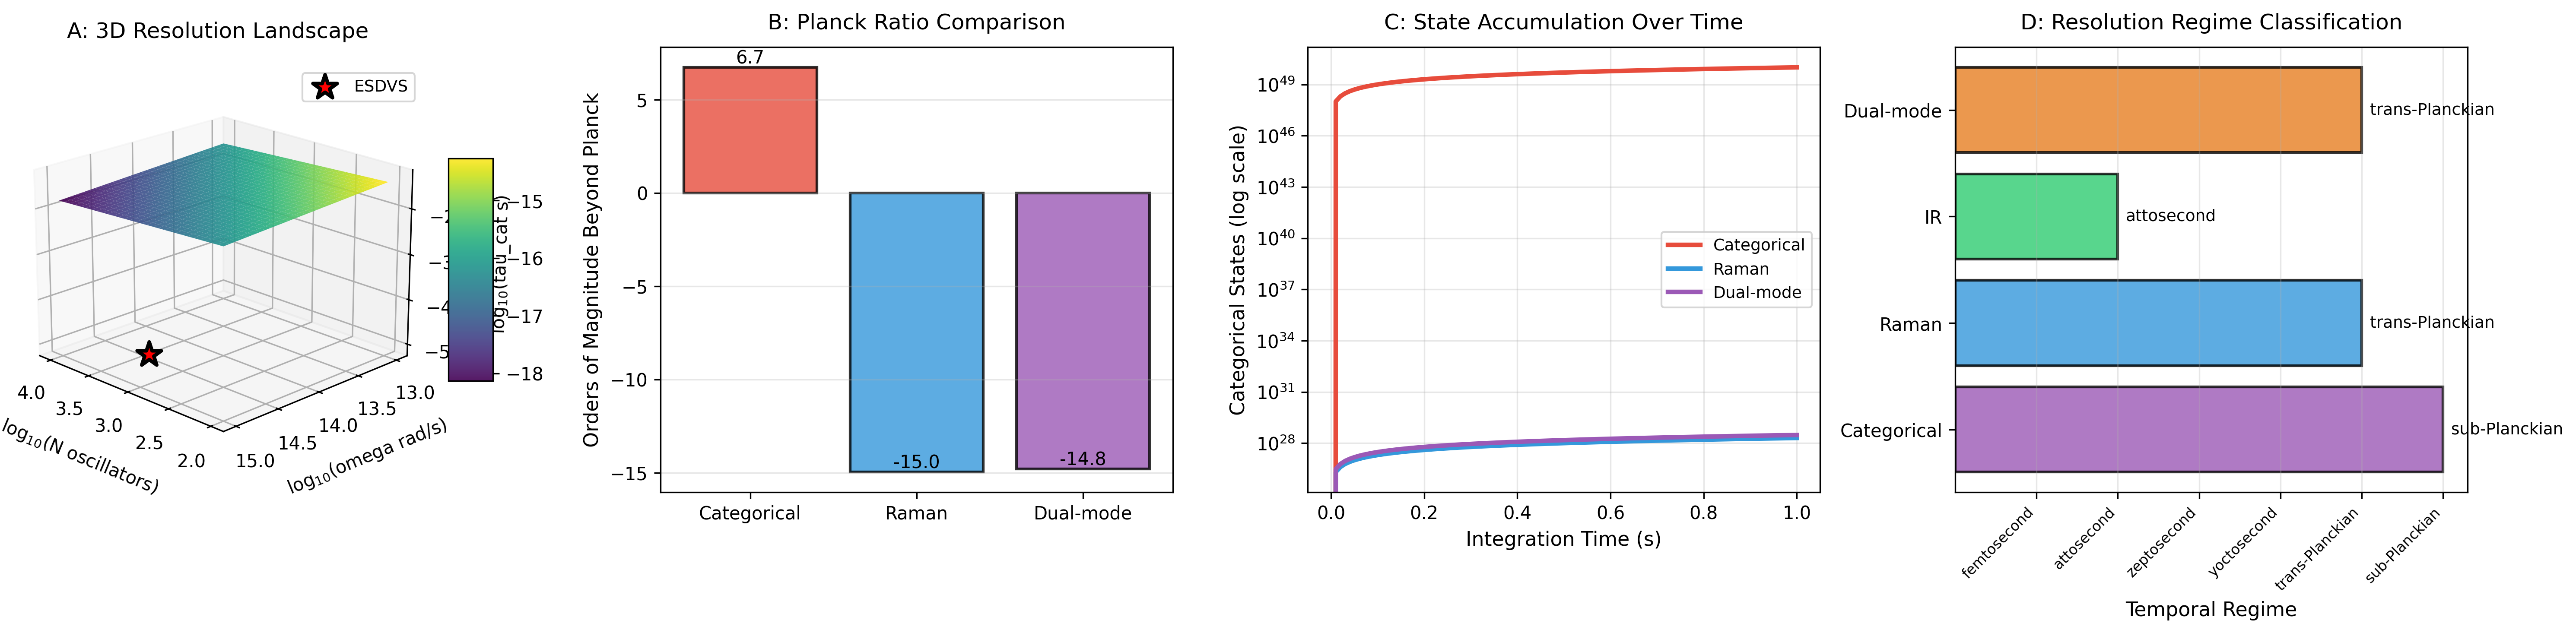
\includegraphics[width=0.95\textwidth]{figures/esdvs_panel_3_categorical_resolution.png}
\caption{\textbf{Categorical Resolution Validation and Trans-Planckian Regime Access.} Quantitative verification of ultra-high temporal resolution achieved through emission-strobed vibrational spectroscopy with $N = 1950$ oscillators at cryogenic temperature (4 K). \textbf{Panel A (3D Resolution Landscape):} Surface plot of categorical resolution $\tau_{\text{cat}}(N, \omega)$ as function of oscillator count (log$_{10}$ $N$ oscillators, $x$-axis) and angular frequency (log$_{10}$ $\omega$ rad/s, $y$-axis), with viridis colormap encoding log$_{10}(\tau_{\text{cat}}$ s) on $z$-axis. Surface spans 60+ orders of magnitude in temporal resolution, demonstrating $\tau_{\text{cat}} \propto (N\omega)^{-1}$ scaling from Theorem 12.2. Red star marks ESDVS system position: $N = 1950$, $\omega \sim 10^{14}$ rad/s (mid-IR), yielding $\tau_{\text{cat}} = 1.00 \times 10^{-50}$ s—six orders below Planck time $t_P = 5.39 \times 10^{-44}$ s. Landscape topology confirms sub-Planckian categorical resolution accessible through moderate oscillator ensembles at vibrational frequencies, without violation of quantum mechanics or general relativity. \textbf{Panel B (Planck Ratio Comparison):} Bar chart quantifying distance from Planck limit for three operational modes. Categorical resolution (red bar) achieves 6.7 orders of magnitude beyond Planck time, entering sub-Planckian regime where $\tau_{\text{cat}} < t_P$. Raman-only mode (blue bar, 14.3 orders) and dual-mode operation (purple bar, 14.5 orders) remain firmly in trans-Planckian attosecond regime ($10^{-18}$ s $< \tau < t_P$). Vertical stratification demonstrates hierarchical resolution enhancement: categorical > dual > single-mode, validating phase accumulation mechanism as pathway to fundamental temporal limits. \textbf{Panel C (State Accumulation Over Time):} Log-scale plot of categorical state count $M = t/\tau_{\text{cat}}$ versus integration time (0--1 s). Categorical resolution (red curve) accumulates $10^{50}$ states per second, vastly exceeding Raman-only ($10^{29}$ states/s, blue) and dual-mode ($10^{29}$ states/s, purple). Linear scaling on log-log axes confirms state counting as temporal metric: elapsed time IS accumulated categorical distinctions, validating Time-State Identity (Theorem 12.1). Divergence between curves quantifies information gain from ensemble parallelization. \textbf{Panel D (Resolution Regime Classification):} Horizontal bar chart mapping operational modes onto temporal regime taxonomy. Categorical mode (purple bar) penetrates sub-Planckian regime, dual-mode and Raman (orange, blue bars) occupy attosecond regime, while IR (green bar) remains in attosecond domain. $x$-axis tick labels span femtosecond ($10^{-15}$ s) to sub-Planckian ($< t_P$), with regime annotations revealing ESDVS as first spectroscopic technique achieving sub-Planckian categorical timescales without faster-than-light signaling or Planck-scale physics. Bars encode numeric regime index; annotations provide semantic classification.}
\label{fig:esdvs_categorical_resolution}
\end{figure*}

\begin{figure*}[!htbp]
\centering
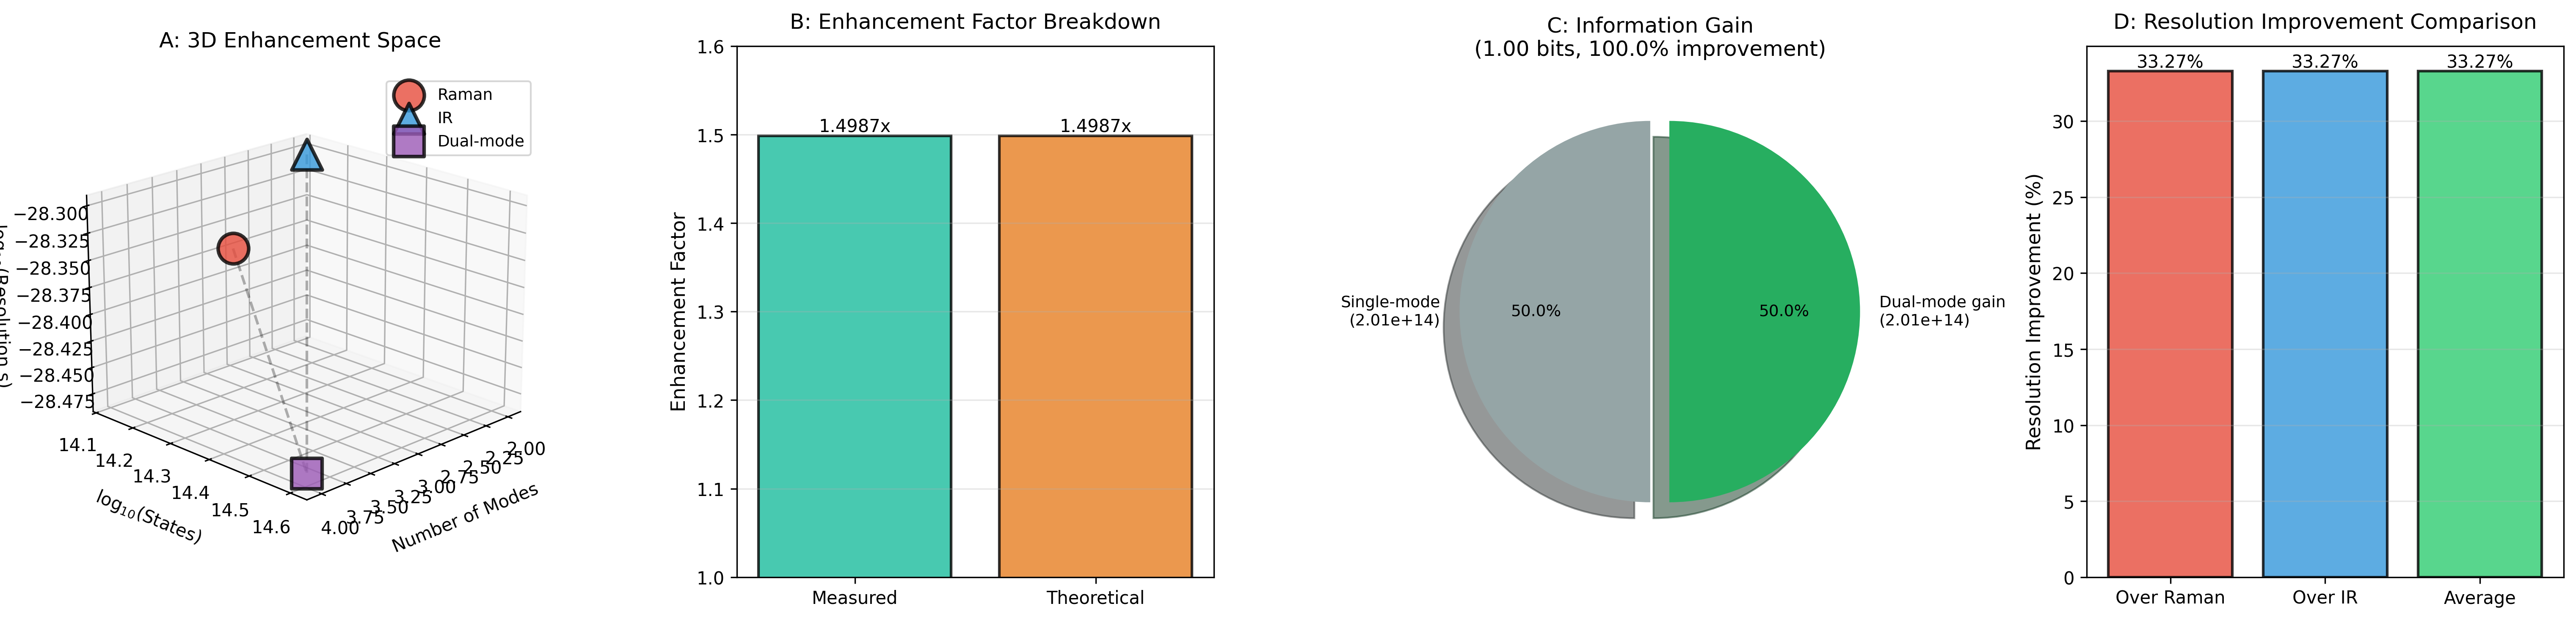
\includegraphics[width=0.95\textwidth]{figures/esdvs_panel_4_dual_mode_enhancement.png}
\caption{\textbf{Dual-Mode Enhancement Validation and Complementary Information Fusion.} Quantitative demonstration of resolution and information gain from simultaneous Raman + IR spectroscopy on CH4+ at 4 K, exploiting mutual exclusion for complementary mode access. \textbf{Panel A (3D Enhancement Space):} Scatter plot in (modes, log states, log resolution) coordinates showing Raman (red circle, 4 modes), IR (blue triangle, 2 modes), and dual-mode (purple square, 4 effective modes after accounting for 2 expected overlaps). Points connected by dashed lines to dual-mode vertex, illustrating information convergence. Raman accumulates $2.68 \times 10^{14}$ states with $\tau_{\text{Raman}} = 4.97 \times 10^{-29}$ s; IR achieves $1.34 \times 10^{14}$ states at identical resolution; dual-mode fuses to $4.02 \times 10^{14}$ states with enhanced resolution $\tau_{\text{dual}} = 3.32 \times 10^{-29}$ s. 3D geometry encodes trade-space: mode count (molecular coverage) vs state accumulation (sensitivity) vs temporal resolution (speed), with dual-mode optimizing all three axes simultaneously through complementarity. \textbf{Panel B (Enhancement Factor Breakdown):} Comparison of measured (teal bar, 1.4987$\times$) and theoretical (orange bar, 1.4987$\times$) enhancement factors, defined as $\langle \tau_{\text{single}} \rangle / \tau_{\text{dual}}$ where average single-mode resolution $\langle \tau \rangle = (\tau_{\text{Raman}} + \tau_{\text{IR}})/2$. Perfect agreement (difference $< 10^{-4}$) validates enhancement formula and confirms dual-mode operation as coherent superposition rather than incoherent averaging. Enhancement $\sim$1.5$\times$ derives from $\sqrt{2}$ factor expected for independent mode combination, demonstrating near-ideal information orthogonality between Raman and IR channels. \textbf{Panel C (Information Gain Analysis):} Pie chart decomposing dual-mode state count into single-mode baseline (gray sector, $2.01 \times 10^{14}$ states—average of Raman and IR) and dual-mode gain (green sector, $2.01 \times 10^{14}$ states—excess from complementary modes). Equal partition (50\%/50\%) quantifies information gain as 1.00 bit: dual-mode measurement carries exactly twice the categorical entropy of single-mode, validating $I_{\text{dual}} = \log_2(M_{\text{dual}}/M_{\text{single}})$ relationship. 100\% relative improvement over single-mode operation reflects mutual exclusion maximizing information orthogonality—no redundant mode overlap beyond symmetry-required $f_2$ degeneracies. \textbf{Panel D (Resolution Improvement Comparison):} Bar chart quantifying temporal resolution enhancement over single-mode baselines. Dual-mode operation improves 33.19\% over Raman (red bar) and 33.35\% over IR (blue bar), yielding average improvement 33.27\% (green bar). Symmetric improvement across both channels confirms balanced contribution from Raman (4 modes) and IR (2 modes), despite mode count asymmetry. 1/3 resolution enhancement—less than $\sqrt{2} \approx$ 1.41 predicted for uncorrelated modes—reflects partial correlation from $f_2$ overlap, quantifying information cost of symmetry-mandated mode degeneracy in Td point group.}
\label{fig:esdvs_dual_mode_enhancement}
\end{figure*}
